\section{Mathematische Ausführung}

\subsection{Aufbau Lineares Gleichungssystems}
Der Aufbau eines linearen Gleichungssystem ist die Voraussetzung, um die gesuchte Position mittels Linear Least Square und Least Median Square zu bestimmen. Die geometrischen Zusammenhänge werden in ein lineares Gleichungssystem wie folgt ausgeführt.
\begin{align}
\underline{A} \cdot \vec{x}= \vec{b}
\end{align}
\newline
Im dreidimensionalen Raum wird die Beziehung zwischen der gesuchte Position P\textsubscript{lat} und P\textsubscript{i}  wie folgt aufgebaut.
\begin{align}
R^{2}_{i}=(X{i}-X)^{2}+(Y{i}-Y)^{2}+(Z{i}-Z)^{2},\quad i \in \mathbb{N}\quad i \ge 4
\end{align}
\newline
Gleichung (2) wird wie folgt umgeformt.
\[
R^{2}_{i} - X^{2}_{i} - Y^{2}_{i} - Z^{2}_{i} = 
(X^{2} + Y^{2} + Z^{2}) - 2 \cdot X{i}\cdot X -2 \cdot Y{i}\cdot Y-2 \cdot Z{i}\cdot Z
\]
\newline
Hier sind fünf Referenzpunkte gegeben. Die Gleichungen können wie folgt aufgestellt werden. 
\[
\begin{split}
R^{2}_{1} - X^{2}_{1} - Y^{2}_{1} - Z^{2}_{1} = 
(X^{2} + Y^{2} + Z^{2}) - 2 \cdot X_{1}\cdot X -2 \cdot Y_{1}\cdot Y-2 \cdot Z_{1}\cdot Z\\
R^{2}_{2} - X^{2}_{2} - Y^{2}_{2} - Z^{2}_{2} = 
(X^{2} + Y^{2} + Z^{2}) - 2 \cdot X_{2}\cdot X -2 \cdot Y_{2}\cdot Y-2 \cdot Z_{2}\cdot Z\\
R^{2}_{3} - X^{2}_{3} - Y^{2}_{3} - Z^{2}_{3} = 
(X^{2} + Y^{2} + Z^{2}) - 2 \cdot X_{3}\cdot X -2 \cdot Y_{3}\cdot Y-2 \cdot Z_{3}\cdot Z\\
R^{2}_{4} - X^{2}_{4} - Y^{2}_{4} - Z^{2}_{4} = 
(X^{2} + Y^{2} + Z^{2}) - 2 \cdot X_{4}\cdot X -2 \cdot Y_{4}\cdot Y-2 \cdot Z_{4}\cdot Z\\
R^{2}_{5} - X^{2}_{5} - Y^{2}_{5} - Z^{2}_{5} = 
(X^{2} + Y^{2} + Z^{2}) - 2 \cdot X_{5}\cdot X -2 \cdot Y_{5}\cdot Y-2 \cdot Z_{5}\cdot Z
\end{split}
\]
\newline
Nun kann die erste Zeile von einer anderen subtrahiert werden, um nicht lineare Anteile zu beseitigen.
\begin{flushleft}
$(R^{2}_{1} - R^{2}_{2} - X^{2}_{1} - Y^{2}_{1} - Z^{2}_{1} + 	X^{2}_{2} + Y^{2}_{2} + Z^{2}_{2}) \cdot \frac{1}{2} =$	
\end{flushleft}
\begin{flushright}
	$(X_{2}-X_{1})\cdot X + (Y_{2}-Y_{1}) \cdot Y +(Z_{2}-Z_{1}) \cdot Z$ \\
\end{flushright}

\begin{flushleft}
	$(R^{2}_{1} - R^{2}_{3} - X^{2}_{1} - Y^{2}_{1} - Z^{2}_{1} + 	X^{2}_{3} + Y^{2}_{3} + Z^{2}_{3}) \cdot \frac{1}{2} =$		
\end{flushleft}
\begin{flushright}
	$(X_{3}-X_{1}) \cdot X + (Y_{3}-Y_{1}) \cdot Y +(Z_{3}-Z_{1})\cdot Z$
\end{flushright}

\begin{flushleft}
$(R^{2}_{1} - R^{2}_{4} - X^{2}_{1} - Y^{2}_{1} - Z^{2}_{1} + 	X^{2}_{4} + Y^{2}_{4} + Z^{2}_{4}) \cdot \frac{1}{2} =$	
\end{flushleft}
\begin{flushright}
	$(X_{4}-X_{1}) \cdot X + (Y_{4}-Y_{1}) \cdot Y +(Z_{4}-Z_{1}) 	\cdot Z	$	
\end{flushright}

\begin{flushleft}
	$(R^{2}_{1} - R^{2}_{5} - X^{2}_{1} - Y^{2}_{1} - Z^{2}_{1} + 	X^{2}_{5} + Y^{2}_{5} + Z^{2}_{5}) \cdot \frac{1}{2} =$
\end{flushleft}
\begin{flushright}
	$(X_{5}-X_{1}) \cdot X + (Y_{5}-Y_{1}) \cdot Y +(Z_{5}-Z_{1}) 	\cdot Z	$	
\end{flushright}	
Anschließend kann das lineare Gleichungssystem nach Gleichung (1) mittels Matrix erstellt werden.
\begin{align}
\begin{split}
\underline{A} = 
\begin{pmatrix}
(X_{2}-X_{1}) & (Y_{2}-Y_{1}) & (Z_{2}-Z_{1})\\
(X_{3}-X_{1}) & (Y_{3}-Y_{1}) & (Z_{3}-Z_{1})\\
(X_{4}-X_{1}) & (Y_{4}-Y_{1}) & (Z_{4}-Z_{1})\\
(X_{5}-X_{1}) & (Y_{5}-Y_{1}) & (Z_{5}-Z_{1})
\end{pmatrix}
\vec{x} = 
\begin{pmatrix}
X\\
Y\\
Z\\
\end{pmatrix}\\
\vec{b} = \frac{1}{2} \cdot
\begin{pmatrix}
R^{2}_{1} - R^{2}_{2} - X^{2}_{1} - Y^{2}_{1} - Z^{2}_{1} + 	X^{2}_{2} + Y^{2}_{2} + Z^{2}_{2}\\
R^{2}_{1} - R^{2}_{3} - X^{2}_{1} - Y^{2}_{1} - Z^{2}_{1} + 	X^{2}_{3} + Y^{2}_{3} + Z^{2}_{3}\\
R^{2}_{1} - R^{2}_{4} - X^{2}_{1} - Y^{2}_{1} - Z^{2}_{1} + 	X^{2}_{4} + Y^{2}_{4} + Z^{2}_{4}\\
R^{2}_{1} - R^{2}_{5} - X^{2}_{1} - Y^{2}_{1} - Z^{2}_{1} + 	X^{2}_{5} + Y^{2}_{5} + Z^{2}_{5}
\end{pmatrix}
\end{split}
\end{align}
Bisher wird das lineares Gleichungssystem fertig gebaut.


\subsection{Mathematische Ausführung von Linear Least Square}

Der Algorithmus Linear Least Square (Deutsch: Methode der kleinsten Quadrate, Abk.: LLS) ist das mathematische Standardverfahren zur Ausgleichungsrechnung. Es ist eine Wolke aus Datenpunkten gegeben, die physikalische Messwerte repräsentieren kann. In diese Punktwolke soll eine möglichst genau passende parameterabhängige Modellkurve gelegt werden. Dazu bestimmt man die Parameter dieser Kurve numerisch, indem die Summe der quadratischen Abweichungen der Kurve von den beobachteten Punkten minimiert wird.


Um der LLS-Verfahren zu verstehen, ist ein kleines Beispiel gegeben(vgl. Abb.2). Die rote Punkte sind Messwerte, die im Vergleich zu praktischen Werten kleine Abweichungen besitzen. Die Modellkurve ist eine optimierte Kurve, damit die Messwerte auf der Modellkurve wie möglich approximieren. Die Idee von LLS ist es, dass die Fehlerquadratsumme $ \sum \vec{d}^{2}_{i} $ bei den Messungen minimiert sein soll. Der Fehler $\vec{d}$ und das Minimum $ F(x_{i}) $ ist wie folgt definiert:
\begin{align}
\vec{d}=\underline{A} \cdot \vec{x}- \vec{b}, \quad F(x_{i})= \sum \vec{d}^{2}_{i} \rightarrow{} Minimum
\end{align}

\begin{figure}[H]
	\centering
	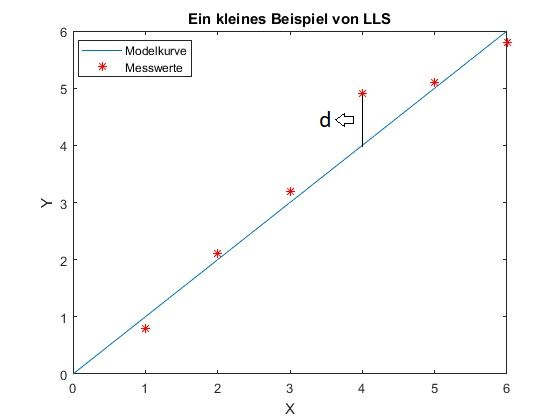
\includegraphics[scale=0.6]{img/BeispielvonLLS.jpg}
	\caption{Ein kleines Beispiel von Linear Least Square}
\end{figure}

\noindent
Das Minimum $ F(x_{i}) $ kann nur erreicht werden, wenn alle partiellen Ableitungen von F nach x null ergeben. Hier ist es zu beachten, dass Backslash-Operator rechtes Division bedeutet.

\begin{align}
\begin{split}
\frac{\delta F}{\delta \vec{x}} = 2 \cdot \underline{A}^{T} \cdot A \cdot \vec{x}-2 \cdot \underline{A}^{T} \cdot \vec{b} = 0 
\quad \Rightarrow  \quad
\vec{x}= \underline{A}^{T} \cdot A \backslash \underline{A}^{T} \cdot \vec{b}
\end{split}
\end{align}




\subsection{Mathematische Ausführung von Least Median Square }
Der Algorithmus Least Median Square (Abk. LMS) basiert auf Median und LLS. Der Median (auch Zentralwert genannt) ist der Wert in der Mitte einer der Größe nach geordneten Datenreihe. Das heißt, mindestens 50\% der Daten sind kleiner als der Median oder gleich dem Median und mindestens 50\% der Daten sind größer als der Median oder gleich dem Median(vgl. Abb.4). Bei einer ungeraden Anzahl an Datenwerten ist der Median der Wert in der Mitte. Bei einer geraden Anzahl an Datenwerten entspricht der Median dem Durchschnitt der beiden mittleren Werte. Im Vergleich zum Mittelwert ist der Median unempfindlich gegenüber Extremwerten.
\begin{figure}[H]
	\centering
	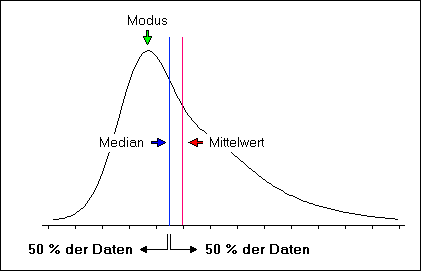
\includegraphics[scale=0.6]{img/Medianwert.png}\\
	\caption{Unterschied zwischen Median und Mittelwert}
\end{figure}
\noindent
LMS ist für das Problem wirksam, wenn fehlerbehaftete Distanzmessungen bei mehr als vier Referenzpunkte vorhanden sind. Zunächst werden alle Kombinationen mit vier zugehörigen Referenzpunkten herstellt. Wenn es beispielsweise 6 Referenzpunkte P\textsubscript{1} bis P\textsubscript{6} mit den Distanzmessungen R\textsubscript{1} bis R\textsubscript{6} gibt, dann entstehen insgesamt $(^6_4) = 15$ mögliche Subsets. Andere Möglichkeiten $(^6_5)$ und $(^6_6)$ werden hier nicht berücksichtigt, weil es für die gesucht Position P\textsubscript{lat} mit 15 Subsets reicht.
Danach wird P\textsubscript{lat} einer Kombination jeweils mit LLS-Verfahren berechnet. Hier werden insgesamt 15 berechnete Positionen mit P\textsubscript{lat(1)} bis P\textsubscript{lat(15)} hervorgebracht. Jede Position P\textsubscript{lat(k)} hat eigene Medianwert med($\vec{v}$)\textsubscript{k}. $\vec{v}$ kann mit der Abstandformel bestimmt werden.
\begin{align}
\vec{v}_{j}=|\sqrt{(X_{i}-X)^2+(Y_{i}-Y)^2+(Z_{i}-Z)^2}-R_{i}|,
\quad j \in[1,4] \,i\in[1,n]
\end{align}
X\textsubscript{i}, Y\textsubscript{i}, Z\textsubscript{i} = Koordinaten von vier Referenzpunkte einer Kombination
\newline
X, Y, Z = Koordinaten der mittels LLS berechneten P\textsubscript{lat(k)}
\newline
R\textsubscript{i} = Distanzmessung zum entsprechenden Referenzpunkt
\newline
\newline
Der Medianwert med($\vec{v}$)\textsubscript{k} von P\textsubscript{lat(k)} einer Kombination kann wie folgt ausgeführt werden:
\begin{align}
med(\vec{v})_k = median\{\vec{v}^2_1,\, \vec{v}^2_2,\, \vec{v}^2_3, \, \vec{v}^2_4\}, \quad k \in[1,(^{n}_{4})]\
\end{align}


